% !TeX program = xelatex
\documentclass{beamer}
\usepackage{etex}
%-------------- template --------------------------------------------------
\usetheme{metropolis}
\metroset{block=fill}
%\usetheme{Boadilla}

% Configuring the foot line
\setbeamertemplate{footline}
{
  \leavevmode%
  \hbox{%
  \begin{beamercolorbox}[wd=.4\paperwidth,ht=2.25ex,dp=1ex,center]{author in head/foot}%
    \usebeamerfont{author in head/foot}\insertshortauthor
  \end{beamercolorbox}%
  \begin{beamercolorbox}[wd=.5\paperwidth,ht=2.25ex,dp=1ex,center]{title in head/foot}%
    \usebeamerfont{title in head/foot}\insertsection
  \end{beamercolorbox}%
  \begin{beamercolorbox}[wd=.1\paperwidth,ht=2.25ex,dp=1ex,right]{date in head/foot}%
    \insertframenumber{} / \inserttotalframenumber\hspace*{2ex} 
  \end{beamercolorbox}}%
  \vskip0pt%
}
% No configuration symbols
\makeatother
\setbeamertemplate{navigation symbols}{}
%----------------------------------------------------------------------------
% context
\AtBeginSection[]
{
    \begin{frame}
        \frametitle{Table of Contents}
        \tableofcontents[currentsection]
    \end{frame}
}
\author[Renato Neves]{Renato Neves}

% logos of institutions
\titlegraphic{
  \begin{textblock*}{5cm}(7.8cm,7.45cm)
     
\includegraphics[scale=0.044]{images/uminho.png}\hspace*{.85cm}~%
  \end{textblock*}
  \begin{textblock*}{5cm}(9.8cm,7.45cm)
    
\includegraphics[scale=0.4]{images/haslab.pdf}
  \end{textblock*}
}

% no date
\date{}


%----------------------------------------------------------------------------
\usepackage{graphicx,amsmath}
\usepackage{stmaryrd} % cf. interleave
\usepackage{booktabs}
\usepackage{amscd}
\usepackage[absolute,overlay]{textpos} % this is for textblock
\usepackage{tikz}
\usetikzlibrary{arrows.meta, calc, fit, tikzmark}
\usepackage{pgfplots}
\usepackage{alltt}
\usepackage{listings}

\def\pvo#1#2{\langle \! \! \! \langle #1 \rangle \! \! \! \rangle\, #2}
\def\uppaal{\textsc{Uppaal}}
\def\cc#1{\mathcal{C}(#1)}
\def\TL#1{\mathcal{T}(#1)}
\input{macros/macros}


\begin{document}

\title{Verification of Timed Systems}

\frame[plain]{\titlepage}

%----------------------------------------------------------------------------------
\begin{slide}{The satisfaction problem}

        Given a system $S$ and a property $\varphi$ show
        that
        \[
                S
                \qquad
                \models \qquad \varphi
        \]


        \medskip
        The choice of which \alert{logical language} to use for
        writing $\varphi$ depends on the underlying computational paradigm
\end{slide}

\begin{slide}{A logical language for timed systems}

        Variant of \alert{Computation Tree Logic} with two types of formulae
        \begin{center}
                \fbox{ 
                        description of \alert{state} and 
                        \alert{path} properties 
                }
        \end{center}
\end{slide}

\begin{frame}{State formulae}

        \begin{block}{Grammar}
        $
        \Psi\; ::=\; \ell ~|~ c ~|~ \texttt{deadlock} ~|~ \texttt{not~}\Psi \mid \Psi \texttt{ and }\Psi 
        $
        \end{block}

        We can thus express \alert{current locations} $\ell$, 
        \alert{clock constraints} $c \in \mathcal{C}(C)$, 
        and the presence of \alert{deadlocks}
\end{frame}

\begin{slide}{Back to the annoying lamp}

  \centering
  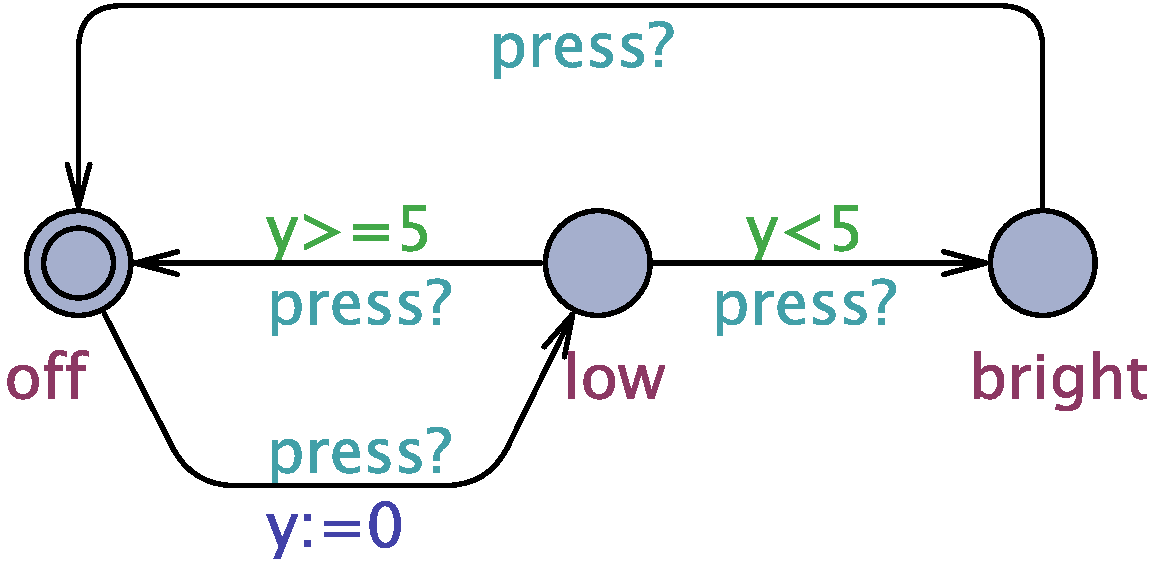
\includegraphics[scale=0.30]{./images/Lamp}

  \begin{block}{Exercise}
          Write formulae for the following statements
  \begin{enumerate}
    \item The lamp is on \texttt{low} mode
    \item Not \texttt{off} and $y>25$
    \item If it is \texttt{low} or \texttt{bright} then $y\leq 3600$
  \end{enumerate}
  \end{block} 
\end{slide}

\begin{slide}{Path Formulae}
\newcommand{\Boxc}{\dgold{\Box}}
\newcommand{\Diamondc}{\dgold{\Diamond}}
\newcommand{\Ac}{\dkb{A}}
\newcommand{\Ec}{\dkb{E}}

\begin{block}{Grammar}
$\Pi\; ::=\;  \Ac \Boxc\, \Psi\, \mid\, \Ac\Diamondc\, \Psi\, \mid\, \Ec \Boxc\, \Psi\, \mid\, \Ec \Diamondc\, \Psi\, \mid\,  \Phi\, \leadsto\, \Psi
$
\end{block}

\dkb{$A$, $E$} quantify (universally / existentially) over paths

\dgold{$\Box$, $\Diamond$} quantify (universally / existentially) over
states in a path

\bigskip
Paths are seen as possible system executions
\end{slide}

\begin{slide}{Path Formulae in Pictures}
\centering

~\\
\begin{tabular}{cc}
  \Large $A \Box\, \varphi$ & \Large $A \Diamond \, \varphi$ \\
 
\includegraphics[width=2.8cm]{./images/AA.jpg} &
 \hspace{1cm} 
\includegraphics[width=2.8cm]{./images/AE.jpg}
\end{tabular}

~\\[2mm]

% \begin{block}{$E \Box\, \varphi$ and $E \Diamond\, \varphi$}
\begin{tabular}{cc}
  \Large $E \Box\, \varphi$ & \Large $E \Diamond\, \varphi$ \\
 
\includegraphics[width=2.8cm]{./images/EA.jpg} &   \hspace{1cm} 
\includegraphics[width=2.8cm]{./images/EE.jpg}
\end{tabular}
% \end{block}
\end{slide}

\begin{slide}{Safety properties}

        \begin{block}{$A \Box\, \varphi \hspace{0.5cm} E \Box\, \varphi$}
        Something bad will \alert{\underline{never}} happen, \eg\ 

\begin{itemize}
\item Temperature will never exceed the prescribed threshold
\item System never reaches a deadlock
\item At least one execution with no deadlocks
\end{itemize}

\end{block}

\end{slide}

\begin{slide}{Reachability properties}

\begin{block}{$E \Diamond\, \varphi$}

        Something good \alert{\underline{can}} happen, \eg\

	\begin{itemize}
                \item All adventurers reach the other side
                \item All adventurers reach the other side in $\leq$ 17 minutes
	\end{itemize}

\end{block}

\end{slide}


\begin{slide}{Path formulae}

        For all paths if $\varphi$ holds at some point then $\psi$ will also
        hold later on

\small \centering

\begin{center}
        \Large $\phi\, \leadsto\, \psi \stackrel{\text{abv}}{=}
        A \Box \, (\phi \to A \Diamond \psi)$ \\[2mm]
\end{center}

\includegraphics[width=5cm]{./images/LeadsTo.jpg} 
\end{slide}


%----------------------------------------------------------------------------------
\begin{slide}{Liveness Properties}

\begin{block}{$A\, \Diamond\, \phi \hspace{0.5cm} \phi\, \leadsto \, \psi$}
        If something happens then something \alert{good}
        \alert{\underline{eventually}} happens
\begin{itemize}
	\item When pressing ON the
		television will eventually turn on
        \item If the philosopher requests a fork she will 
                get it
        \item If the plane asks to land it will eventually land
\end{itemize}

\end{block}

\end{slide}

\begin{frame}{Exercises}
	Write the sentences below in CTL
	\begin{enumerate}
		\item The system never enters in deadlock
		\item The location $\ell$ is reachable
		\item In all executions we reach location $\ell$
		\item If we reach location $\ell$ we will inevitably reach
			location $s$
		\item There exists at least one execution where variable
			\texttt{i} is always below or equal \texttt{10}
		\item The two philosophers never eat at the same time
	\end{enumerate}
\end{frame}

\begin{frame}{Back to the Annoying Lamp}

        \centering
        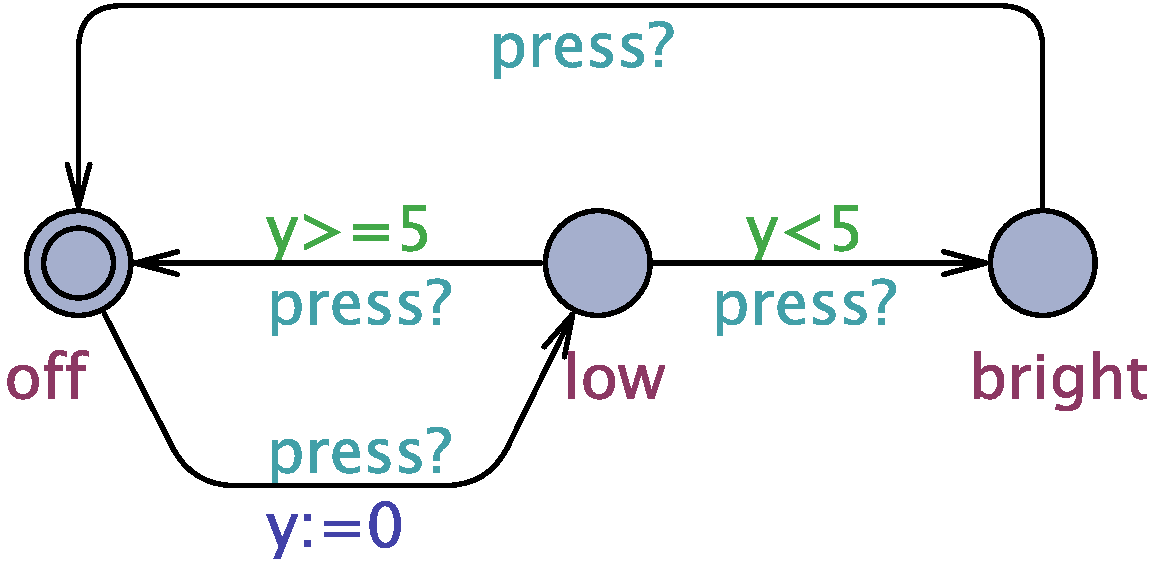
\includegraphics[scale=0.25]{./images/Lamp.pdf}

        \begin{block}{Exercise}
	\begin{enumerate}
                \item The lamp can become bright;
                \item The lamp will eventually become bright;
                \item The lamp can never be on for more than 3600s;
                \item It is possible to never turn on the lamp;
                \item Whenever the light is bright, the clock $y$
                        is non-zero;
                \item Whenever the light is bright it will eventually
                        become off.
	\end{enumerate}
        \end{block}
\end{frame}

\section{Chapter's Conclusion}

\begin{frame}{Key Takeaways}

        Communicating systems as \tikzmark{z1} \alert{timed automata} 
        \tikzmark{z2}

        \begin{tikzpicture}[overlay,remember picture, box/.style
        = {rounded corners}, pin edge={-Stealth,thick, red}] 
        \coordinate (z1) at
        ($({pic cs:z1})+(0.5ex, 1.5ex)$); 
        \coordinate (z2) 
                at ($({pic cs:z2})+(-1.5ex,-0.5ex)$); 
        \node[semitransparent, fit=(z1) (z2),
                pin=below:\tiny{Syntax}]
        {};
        \end{tikzpicture}

        \vspace{0.5cm}
        \alert{Semantics} for rigorous analysis and verification

        \vspace{1cm}
        \alert{UPPAAL} as an important tool of the cyber-physical engineer
\end{frame}

\begin{frame}{Key takeaways}


        \vspace{0.4cm}
        \alert{Time} as the main physical process \dots

        \dots\ others will appear in the next lectures

        \vspace{0.4cm}
        Barely scratched the surface \dots

        \dots\ more about the theory of timed automata 
        in the website
\end{frame}
\end{document}
